\chapter{Pendahuluan}

%---------------------------------------------------------
\section{Latar Belakang}
%---------------------------------------------------------
Dalam perancangan produk perangkat lunak, tentunya kita akan mempertimbangkan tentang siapa yang akan menggunakan perangkat lunak tersebut. Hal ini tetunya harus dilakukan karena kita menginginkan bahwa perangkat lunak yang dibuat memiliki fungsionalitas yang sesuai dengan kebutuhan para penggunanya. Oleh karena itu, dalam sebuah perancangan perangkat lunak diperlukan adanya proses pengumpulan informasi kebutuhan (\textit{requirement gathering}) agar rancangan perangkat lunak yang kita buat sesuai dengan ekspektasi dan kebutuhan pengguna. \\

\noindent
Berbicara tentang \textit{requirement} perangkat lunak, kita mengetahui bahwa seiring berjalannya waktu, jumlah dan tingkat kompleksitas dari \textit{requirement} sebuah perangkat lunak akan semakin meningkat. Hal ini tentunya disebabkan oleh semakin tingginya kebutuhan dan luasnya domain permasalahan para pengguna yang harus ditangani oleh perangkat lunak tersebut. Dampak dari dua hal tersebut pada akhirnya memaksa para pengembang perangkat lunak untuk terus melakukan perubahan (evolusi) terhadap perangkat lunak yang dibuatnya. Apabila proses evolusi perangkat lunak tersebut tidak sebanding dengan peningkatan kebutuhan pengguna, maka para pengguna perangkat lunak tersebut akan berpaling ke perangkat lunak lain yang dinilai dapat memenuhi kebutuhan mereka saat ini. \\

\noindent
Salah satu pendekatan yang dapat digunakan untuk melakukan proses evolusi produk perangkat lunak secara cepat dan efisien adalah dengan menggunakan pendekatan \textit{Software Product Line Engineering} (SPLE). SPLE merupakan sebuah paradigma yang digunakan dalam proses pengembangan perangkat lunak dengan menggunakan konsep \textit{software platform} dan \textit{mass customisation} \citep[p.~14]{pohl2005software}. Dengan menggunakan paradigma ini, proses evolusi produk perangkat lunak dapat dilakukan dengan melihat aspek \textit{commonality} dan \textit{variability} dari komponen-komponen yang ada. Hal ini tentunya akan membuat proses evolusi produk perangkat lunak menjadi lebih cepat dan efisien dikarenakan para pengembang produk perangkat lunak tidak perlu mengembangkan produknya dari awal untuk memenuhi variasi dari kebutuhan yang sama. \\

\noindent
Salah satu teknologi yang dapat digunakan dalam melakukan pengembangan \textit{Software Product Line} (SPL) adalah \textit{Abstract Behavioural Spesification} (ABS). ABS adalah sebuah bahasa pemodelan yang dibuat oleh konsorsium uni eropa sejak tahun 2008 dengan nama proyek \textit{Highly Adaptable and Trustworthy Software using Formal Methods} (HATS). bahasa pemodelan ini didesain khusus memiliki kemampuan untuk melakukan pemodelan fitur dan delta sehingga dapat digunakan untuk membuat SPL. Secara sintaksis, ABS memiliki sintaks yang mirip dengan bahasa pemrograman JAVA. Kemiripan sintaks ABS dengan JAVA sengaja dibuat agar para pengembang perangkat lunak dengan mudah beradaptasi dengan bahasa pemodelan ini \citep{hahnle2013hats}. \\

\noindent
Dalam proses pengembangan perangkat lunak, \textit{code reuse} dan \textit{code maintenance} menjadi hal yang harus diperhatikan dengan baik. Kedua aspek tersebut mendapat perhatian khusus dikarenakan proyek perangkat lunak merupakan proyek yang berkepanjangan (terus berevolusi) dan memerlukan tingkat kolaborasi yang tinggi (terutama untuk perangkat lunak dengan sekala yang besar). Salah satu \textit{best practice} yang digunakan untuk dapat mewujudkan kedua aspek tersebut adalah dengan menggunakan sebuah pendekatan yang bernama \textit{Model-View-Controller} (MVC). MVC merupakan sebuah pendekatan yang digunakan dalam proses perangkat lunak untuk memisahkan antara logika aplikasi, data, dan presentasi \citep{leff2001web} \citep{krasner1988desc}. Dalam penelitian ini, penulis akan membuat sebuah \textit{framework} MVC untuk ABS yang nantinya akan digunakan dalam proses pengembangan SPL berbasis web.

%---------------------------------------------------------
\section{Manfaat Penelitian}
%---------------------------------------------------------
Adapun manfaat dari penelitian yang dilakukan antara lain adalah:
\begin{enumerate}
    \item Memberikan pengetahuan lebih lanjut terkait bagaimana melakukan perancangan dan penerapan pola \textit{Model-View-Controller} dalam melakukan pengembangan SPL berbasis web dengan menggunakan bahasa pemodelan ABS.
    \item Membuktikan bahwa bahasa pemodelan ABS juga dapat digunakan dalam pengembangan aplikasi \textit{frontend} dan bukan hanya untuk aplikasi \textit{backend} yang tidak memiliki \textit{user interface} (seperti yang dilakukan selama ini).
    \item Menghasilkan sebuah \textit{framework} MVC ABS yang dapat digunakan oleh para pengembang perangkat lunak untuk dapat membuat SPL berbasis web dengan menggunakan ABS.
\end{enumerate}

%---------------------------------------------------------
\section{Rumusan Masalah}
%---------------------------------------------------------
\noindent
Berikut ini adalah rumusan masalah dari penelitian yang penulis lakukan:

\begin{enumerate}
    \item Bagaimana strategi yang tepat dalam melakukan pemetaan bahasa pemodelan ABS ke dalam pola Model, View dan Controller dengan tetap mempertahankan kaidah-kaidah yang ada sesuai dengan studi literatur yang telah dilakukan?
    \item Bagaimana strategi implementasi yang dapat dilakukan agar \textit{framework} ABS yang dibuat dapat mendukung fitur \textit{delta modeling} yang dimiliki oleh ABS?
    \item Apakah \textit{framework} yang dibuat dapat mendukung pengembangna SPL berbasis web?
\end{enumerate}

%---------------------------------------------------------
\section{Ruang Lingkup Penelitian}
%---------------------------------------------------------
\noindent
Adapun ruang lingkup dari penelitian ini adalah tentang perancangan dan perumusan strategi pengembangan \textit{framework} MVC SPL berbasis web dengan menggunakan bahasa pemodelan ABS. Harapannya, melalui penelitian ini penulis dapat menghasilkan sebuah \textit{framework} ABS yang dapat digunakan untuk melakukan pengembangan SPL berbasis web dengan menggunakan bahasa pemodelan ABS. Berdasarkan ruang lingkup tersebut, maka poin-poin pengerjaan yang akan dilakukan oleh penulis dalam penelitian ini antara lain adalah:

\begin{enumerate}
    \item Melakukan analisa terhadap sintaks dan aturan-aturan yang berlaku pada bahasa pemodelan ABS untuk kemudian dapat dirumuskan strategi dalam melakukan pemetaan bahasa pemodelan ABS kedalam komponen-komponen \textit{Model, View} dan \textit{Controller}.
    \item Merancang arsitektur dan strategi pengembangan \textit{framewok} ABS agar dapat mendukung fitur \textit{delta modeling} yang dimiliki oleh ABS.
    \item Membuat framework ABS berdasarkan strategi dan rancangan yang telah dilakukan sebelumnya.
\end{enumerate}

%---------------------------------------------------------
\section{Batasan Penelitian}
%---------------------------------------------------------

Dikarenakan adanya keterbatasan dalam hal pengetahuan, waktu pengerjaan dan fokus pengerjaan maka penulis menentukan batasan-batasan penelitian untuk penelitian kali ini yang diantaranya adalah:

\begin{enumerate}
    \item \textit{Framework} yang dibuat belum mendukung akses database karena untuk masalah akses \textit{database} pada ABS sudah menjadi topik penelitian tersendiri.
    \item \textit{Web Server} yang dibuat hanya berupa \textit{web server} sederhana dengan fungsionalitas terbatas pada menerima \textit{HTTP Request}, meneruskan \textit{request} tersebut ke ABS, serta mengirimkan \textit{HTTP Response} yang diberikan oleh ABS ke web browser. Oleh karena itu, penulis tidak akan mempertimbangkan masalah keamanan data, efisiensi dari \textit{web server} ataupun masalah \textit{concurency access} pada \textit{web server}.
    \item Penulis tidak melakukan komparasi antara \textit{framework} MVC yang dibuat dengan \textit{framework} MVC sejenis dikarenakan masih minimnya literatur yang membahas tentang pengembangan \textit{framework} MVC SPL berbasis web untuk bahasa pemodelan ABS.
\end{enumerate}

%---------------------------------------------------------
\section{Kerangka Berpikir}
%---------------------------------------------------------
\noindent
Tujuan utama dari dilakukannya penelitian ini adalah adalah untuk menganalisa dan merancang strategi pengembangan SPL berbasis web dengan menggunakan bahasa pemodelan ABS. Ketika berbicara tentang perangkat lunak berbasis web, tentunya kita juga harus memikirkan bagaimana caranya agar perangkat lunak yang sudah dibuat dapat berjalan di \textit{web server}. Dalam konteks ABS, penulis perlu mencari tahu bagaimana caranya agar ABS dapat berjalan di atas platform JAVA \textit{Application Server} yang sudah ada seperti misalnya Apache Tomcat atau Oracle Glassfish. Apabila ABS tidak dapat dijalankan di atas platform yang sudah ada, maka penulis harus membuat sendiri sebuah \textit{Application Server} yang dapat menjalankan ABS.

\begin{figure}
    \centering
    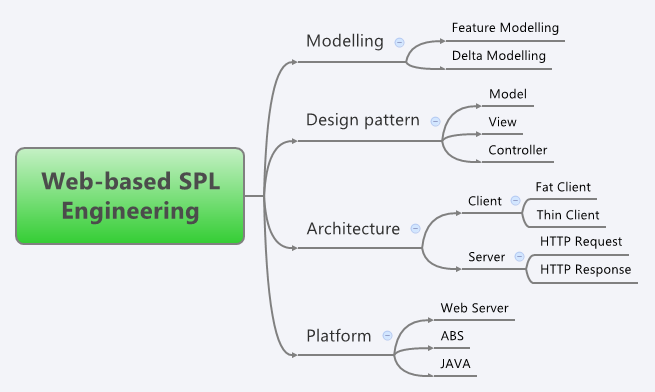
\includegraphics[width=0.8\textwidth]
        {img/kerangka-berpikir.png}
    \caption{Kerangka berpikir}
\end{figure}

\noindent
Setelah penulis mengetahui solusi apa yang harus digunakan agar ABS dapat berjalan di \textit{Application Server}, selanjutnya penulis akan merancang bagaimana pengorganisasian kode yang baik untuk ABS agar sesuai dengan kaidah MVC. Hal ini perlu dilakukan karena nantinya penelitian ini akan menghasilkan sebuah \textit{framework} MVC yang akan digunakan dalam pengembangan SPL berbasis web dengan menggunakan ABS. Dalam hal ini, penulis harus mengkaji terkait peran-peran setiap komponen pada MVC dan kemudian mengimplementasikannya ke ABS. \\

\noindent
Rangkaian proses diatas diharapkan nantinya menghasilkan sebuah framwork MVC yang utuh untuk kemudian diintegrasikan dengan konsep \textit{feature modeling} dan \textit{delta modeling} yang ada di ABS. Hal ini dilakukan agar dapat dihasilkan sebuah framework MVC ABS yang dapat digunakan untuk keperluan pengembangan SPL berbasis web.

%---------------------------------------------------------
\section{Sistematika Penulisan}
%---------------------------------------------------------
berikut adalah sistematika penulisan dari proposal ini:
\begin{itemize}
    \item Bab 1 Pendahuluan \\
    Bab ini berisi tentang latar belakang penelitian, manfaat penelitian, kerangka berpikir, dan sistematika penulisan.
    \item Bab 2 Studi Literatur \\
    Bab ini berisi tentang hasil studi literatur yang dilakukan oleh penulis baik terkait teori-teori dasar yang mendukung penelitian ini ataupun peneletian lain yang masih berkaitan dengan penelitian yang akan dilakukan.
    \item Bab 3 Rumusan Masalah \\
    Bab ini berisi tentang rumusan masalah dari penelitian yang akan dilakukan, ruang lingkup penelitian, serta batasan penelitian.
    \item Bab 4 Perancangan ABS MVC Framework \\
    Bab ini berisi tentang detail rancangan \textit{framework} yang telah penulis buat. Rancangan ini penulis jadikan sebagai landasan dalam melakukan proses pengembangan \textit{framework}.
    \item Bab 5 Pembuatan Halaman Web Menggunakan ABS \\
    Bab ini memaparkan secara kronologis tentang proses eksperimen yang telah dilakukan oleh penulis untuk mencoba sebuah halaman web dengan menggunakan bahasa pemodelan ABS.
    \item Bab 6 Penyusunan ABS MVC Framework \\
    Bab ini memaparkan tentang proses eksperiemen yang penulis lakukan dalam menyusun ABS MVC Framework berdasarkan hasil eksperimen sebelumnya.
    \item Bab 7 Penerapan ABS MVC Framework \\
    Bab ini memaparkan tentang contoh pengembangna perangkat lunak berbasis web dengan menggunakan ABS MVC Framework yang telah dibuat.
    \item Bab 8 Penerapa \textit{delta modeling} pada ABS MVC Framework \\
    Bab ini memaparkan tentang bagimana menerapkan fitur \textit{delta modeling} yang dimiliki oleh ABS dalam menangani perubahan \textit{requirement} pada sistem dengan menggunakan ABS MVC Framework.
    \item Bab 9 Evaluasi \\
    Bab ini memaparkan tentang evaluasi yang penulis lakukan terhadap ABS MVC Framework yang dibuat.
    \item Bab 10 Kesimpulan \\
    Bab ini berisi tentang kesimpulan-kesimpulan yang penulis dapatkan setelah melakukan penelitian ini.
\end{itemize}